\documentclass[12pt]{report}
\usepackage{graphicx}
\usepackage{caption}
\usepackage[english]{babel}
\usepackage{caption}
\usepackage{capt-of}
\usepackage{color, colortbl}
\usepackage[hidelinks]{hyperref}
\usepackage[numbers]{natbib}
\usepackage[nohyperlinks, printonlyused, withpage, smaller]{acronym}
\usepackage[ngerman]{datetime}
\usepackage{chngcntr}
\usepackage{pdfpages}
\usepackage{enumitem}
\usepackage{amsmath}
\usepackage{tikz}
\usepackage[skins]{tcolorbox}
\usepackage{rotating}
\usepackage{framed}
\counterwithin{figure}{section}
\usepackage{lipsum}
\usepackage{float}
\usepackage{listings}
\usepackage{xcolor}
\usepackage{listing}
\usepackage{hyperref}
\usepackage{lscape}
\usepackage{longtable}
\usepackage{multirow}
\usepackage{upquote}
\usepackage{longtable}
\usepackage{booktabs}
\usepackage[titletoc]{appendix}

\colorlet{punct}{red!60!black}
\definecolor{background}{HTML}{EEEEEE}
\definecolor{delim}{RGB}{20,105,176}
\colorlet{numb}{magenta!60!black}

\lstdefinelanguage{json}{
    basicstyle=\normalfont\ttfamily,
    numbers=left,
    numberstyle=\scriptsize,
    stepnumber=1,
    numbersep=8pt,
    showstringspaces=false,
    breaklines=true,
    frame=lines,
    backgroundcolor=\color{background},
    literate=
     *{0}{{{\color{numb}0}}}{1}
      {1}{{{\color{numb}1}}}{1}
      {2}{{{\color{numb}2}}}{1}
      {3}{{{\color{numb}3}}}{1}
      {4}{{{\color{numb}4}}}{1}
      {5}{{{\color{numb}5}}}{1}
      {6}{{{\color{numb}6}}}{1}
      {7}{{{\color{numb}7}}}{1}
      {8}{{{\color{numb}8}}}{1}
      {9}{{{\color{numb}9}}}{1}
      {:}{{{\color{punct}{:}}}}{1}
      {,}{{{\color{punct}{,}}}}{1}
      {\{}{{{\color{delim}{\{}}}}{1}
      {\}}{{{\color{delim}{\}}}}}{1}
      {[}{{{\color{delim}{[}}}}{1}
      {]}{{{\color{delim}{]}}}}{1},
}

\def\frontmatter{%
    \pagenumbering{roman}
    \setcounter{page}{1}
    \renewcommand{\thesection}{\Roman{section}}
}%

\def\mainmatter{%
    \pagenumbering{arabic}
    \setcounter{page}{1}
    \setcounter{section}{0}
    \renewcommand{\thesection}{\arabic{section}}
}%

\def\backmatter{%
    \setcounter{section}{0}
    \renewcommand{\thesection}{\Alph{section}}
}%
\renewcommand{\listfigurename}{\begingroup
    \tocchapter{}
    \tocfile{\listoffigurename}{B Illustration Directory}
\endgroup}

\begin{document}
\frontmatter

\begin{titlepage}
    \newcommand{\HRule}{\rule{\linewidth}{1.5mm}}
    \center{}
    \begin{figure}
        \centering
        
\includegraphics[width=0.5\textwidth]{img/hslogo}\label{pic:Logo}
    \end{figure}

    \begin{center}
    \end{center}

    {\huge Masterproject}\\[0.4cm]
    \begin{center}
    \end{center}
    {\Large Geocoding and Routing with Pelias and Valhalla }\\
    \vfill
    \begin{center}
        {Contributors:}\ \\
        \vspace{0.25\baselineskip}
        {\Large Martin Schmid, Sergej Dechant}
    \end{center}
    \vfill
    \begin{center}
        {\large Expert: Prof.\ Dr.\ von Schwerin }\\
    \end{center}
    \begin{center}
        {\large Expert: Prof.\ Dr.\ Herbort}
    \end{center}
    \begin{center}
        {\large Expert: Prof.\ Dr.\ Goldstein}
    \end{center}
    \vfill
    {\Large \today}

\end{titlepage}

\newpage
\tableofcontents
\mainmatter{}
\newpage
\chapter{Project Presentation and Scope}
% TODO: reorganize, rewrite
% vim:ft=tex

\section{Introduction}
The purpose of this paper is to document the progress of the "junior team" during the first half of the data science project in form of a technical report. Moreover, this report should allow readers to gain an understanding of the topics covered in the data science project as well as be able to reproduce and extend the developed and utilized solutions.
The covered tasks during the first half of the project can be categorized into three main areas:
\begin{enumerate}
\item Infrastructure
\begin{itemize}
\item Set up a virtual machine (Ubuntu Linux)
\item Install and configure Pelias and Elasticsearch
\item Install and evaluate different routing engines
\end{itemize}
\item Data acquisition and preparation
\begin{itemize}
\item Gather postcode data of European countries from different sources
\item Merge postcode data into a single data source for Pelias and Elasticsearch
\end{itemize}
\item Geocodoing and Routing
\begin{itemize}
\item Test geocoding with Pelias based on precalculated two-digit postcode centroids
\item Test routing between two-digit postcode centroids wit a routing engine
\end{itemize}
\end{enumerate}

% vim:ft=tex

\section{Requirements}
The main requirements were to evaluate Pelias as an open source geocoding service and as an alternative to Nominatim as well as to realize routing from one two-digit postcode to another. In order to achieve this it was necessary to build a database of postcodes and create a map of Europe based on data provided by Openstreetmaps, Whosonfirst, Geonames and Postcodeinfo. Furthermore, routing engines as an alternative to Graphhopper had to be evaluated. Last but not least an adequate documentation on how these requirements can be fulfilled and the outcome reproduced had to be written.
\chapter{Pelias}
% vim:ft=tex

\section{Pelias}
\subsection{General}
\subsubsection{Capabilities}
Pelias is a software solution/library used for geocoding. Geocoding is the process of taking input text, such as an address or the name of a place and returning a latitude/longitude location on the Earth's surface for that place.
The "senior team" used Nominatim for geocoding, which is a tool for geocoding just like pelias. One of our main tasks  in the course of the first half of the project was to test and evaluate pelias as an alternative open-source geocoder to Nominatim.

Here are some benefits of the pelias API:
\begin{itemize}
\item Completely open-source and MIT licensed
\item A powerful data import architecture: Pelias supports many open-data projects out of the box but also works great with private data
\item Support for searching and displaying results in many languages
\item Fast and accurate autocomplete for user-facing geocoding
\item Support for many result types: addresses, venues, cities, countries, and more
\item Easy installation with minimal external dependencies
\end{itemize}

As mentioned above, pelias has the ability to import data from many different open-data projects as well as own private data. The importers filter, normalize, and ingest geographic datasets into the Pelias database. Currently there are five officially supported importers:

\begin{itemize}
\item \textbf{OpenStreetMap:} supports importing nodes and ways from OpenStreetMap
\item \textbf{OpenAddresses:} supports importing the hundreds of millions of global addresses collected from various authoritative government sources by OpenAddresses
\item \textbf{Who's on First:} supports importing admin areas and venues from Who's on First
\item \textbf{Geonames:} supports importing admin records and venues from Geonames
\item \textbf{Polylines:} supports any data in the Google Polyline format. It's mainly used to import roads from OpenStreetMap
\item \textbf{Custom Data Importer:} creates a Pelias record for each row in a CSV file. Each row must define a source, latitude, longitude, and either an address, name, or both. This feature was used to import two-digit postcodes into Pelias.
\end{itemize}

\begin{figure}[H]
\centering
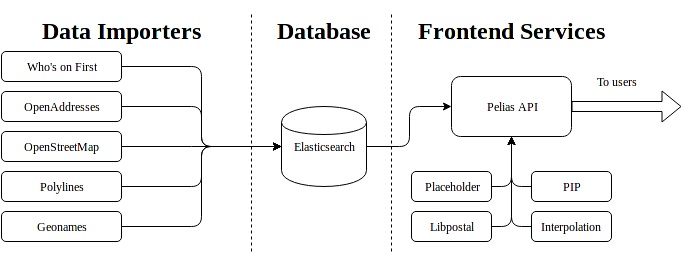
\includegraphics[width=1.0\textwidth]{img/pelias_architecture}
\captionof{figure}{Overview of the pelias architecture}
\label{fig:pelias_architecture}
\end{figure}

\subsubsection{Database}
The underlying datastore that powers the search results and does query-lifting is Elasticsearch. Currently version 2.4 is supported, with plans to support 5.x soon. The developers built a tool called pelias-schema that sets up Elasticsearch indices properly for Pelias.

\subsubsection{Dependencies}
These are software projects that are not used directly but are used by other components of Pelias:
\begin{itemize}
\item \textbf{model:} provide a single library for creating documents that fit the Pelias Elasticsearch schema. This is a core component of Pelias‘ flexible importer architecture
\item \textbf{wof-admin-lookup:} A library for performing administrative lookup using point-in-polygon math. Previously included in each of the importers but now only used by the PIP service.
\item \textbf{query:} This is where most of Elasticsearch’s query generation happens.
\item \textbf{config:} Pelias is very configurable, and all of it is driven from a single JSON file which is called pelias.json. This package provides a library for reading, validating, and working with this configuration. It is used by almost every other Pelias component
\item \textbf{dbclient:} A Node.js stream library for quickly and efficiently importing records into Elasticsearch
\end{itemize}

\subsection{System Requirements}
\subsubsection{Software Requirements}
\begin{itemize}
\item \textbf{Node.js:} Version 8 or newer is required, version 10 is recommended for improved performance.
\item \textbf{Elasticsearch:} Version 2.4 or 5.6
\item \textbf{SQLite:} Version 3.11 or newer
\item \textbf{Libpostal:} Pelias relies heavily on the Libpostal address parser. Libpostal requires about 4GB of disk space to download all the required data.
\end{itemize}

\subsubsection{Hardware Requirements}
\begin{itemize}
\item At a minimum 50GB disk space to download, extract, and process data
\item 8GB RAM for a local build, 16GB+ for a full planet build. Pelias needs a little RAM for Elasticsearch, but much more for storing administrative data during import
\item As many CPUs as possible. There's no minimum, but Pelias builds are highly parallelizable, so more CPUs will help make it faster.
\end{itemize}

Actual system used for the project (Europe build):
\begin{itemize}
\item 1 virtual machine (Ubuntu Linux) with 64 GB RAM, 500GB HDD, 4 CPU cores
5
\item RAM utilization is at ~30 GB, however during the import of openstreetmaps data and calculating polylines from it up to 40 GB of RAM were used. Imports and calculations maxed out all CPU cores. It is possible to reduce the required amount of RAM for imports and calculations. However, this requires splitting up openstreetmap files in smaller files with other tools beforehand.
\item Including “raw data” (before the import and calculations) around 400GB of data are persisted on HDD, Elasticsearch uses ~100GB.
\end{itemize}
\section{Installation and Configuration}
Pelias can be installed with Docker Images, manually from scratch or with Kubernetes. For testing purposes installing Pelias using Docker Images is strongly recommended by the developers \cite{Simioni2018b}. Pelias can also be installed manually from scratch, but due to the large amount of dependencies this is not recommended by the developers. To use Pelias in production, the development team suggests an installation with Kubernetes, which is by far the most tested and best way to install and use Pelias in production according to the development team.

\subsection{Installation with Docker}
On the virtual machine Pelias was installed and maintained with Docker and Docker-Compose. Install Docker and Docker-Compose:
\begin{lstlisting}[language=bash,breaklines=true]
sudo apt-get update
sudo apt-get install \
apt-transport-https \
   ca-certificates \
	curl \
	gnupg-agent \
	software-properties-common
curl -fsSL https://download.docker.com/linux/ubuntu/gpg | sudo apt-key add -
sudo add-apt-repository \ "deb [arch=amd64] https://download.docker.com/linux/ubuntu \
	$(lsb_release -cs) \ stable"
sudo apt-get update
sudo apt-get install docker-ce docker-ce-cli containerd.io
sudo groupadd docker
sudo usermod -aG docker $USER
sudo systemctl enable docker
sudo curl -L "https://github.com/docker/compose/releases/download/1.24.0/docker-compose-$(uname -s)-$(uname -m)" -o /usr/local/bin/docker-compose
sudo chmod +x /usr/local/bin/docker-compose
\end{lstlisting}
Afterwards Pelias can be installed by cloning Pelias' git repository. In this repository Pelias' developers provide example projects (e.g. Beligum, Portland Metro, etc.). Pelias' "planet" project was used as a starting point for a Europe build. For this Pelias was forked on Github and cloned onto the VM. The project can be found in the following folder:
\begin{lstlisting}[language=bash,breaklines=true]
/home/dataproject/git/pelias-docker/projects/Europe
\end{lstlisting}
In order to build and run Pelias with data for Europe four configuration files in this folder are needed:
\begin{enumerate}
\item .env
\item Elasticsearch.yml
\item pelias.json
\item docker-compose.yml
\end{enumerate}

The files can be found in the appendix on page \pageref{Dicf}.

In .env DATA{\_}DIR and DOCKER{\_}USER are important entries/variables. DATA{\_}DIR specifies where Pelias will store downloaded data and build its other services. DOCKER{\_}USER specifies the user id. This user id will be used for accessing files on the host filesystem in DATA{\_}DIR since Pelias' processes run as non-root users in containers.
In Elasticsearch.yml both thread pool sizes had to be increased since the default values were too small. Pelias importers delivered too much data concurrently for Elasticsearch which resulted in corrupted data.
In pelias.json all Pelias services are configured. These services run as docker containers. Therefore, it is not necessary to provide complete full paths on the host filesystem or IP/DNS addresses. Paths are mapped to the paths provided in the docker compose file  and .env file. Docker has its own networking and DNS. Services in a docker network can be addressed by using docker compose service names as well as container names and ids. Container ports can be mapped to host ports.
The variables DOCKER{\_}USER and DATA{\_}DIR in docker-compose.yml are mapped to the corresponding entries in .env. Inside containers pelias.json is made available in /code/pelias.json. Ports are mapped in the following way:
hostport:containerport.
The "image" directive tells docker from where it has to pull the container image. In this case all images are pulled from the Pelias repository on Docker-Hub. After the colon a tag is specified (e.g. master or a version/hash). If no tag is provided, the latest version will be pulled.
With this configuration it is possible to build Europe completely with the following commands and order (cd to Europe project folder first):
\begin{lstlisting}[language=bash,breaklines=true]
pelias compose pull
pelias elastic start
pelias elastic wait
pelias elastic create
pelias download all
pelias prepare all
pelias import all
pelias compose up
\end{lstlisting}

\subsection{Installation from scratch}
In order to do a clean installation of the pelias service and its dependencies on a production server at a later point in time we decided to try the installation from scratch and wrote an installation guide. The complete guide can be found in the appendix on page \pageref{Pfsig}. We did the installation on a Linux VM running Ubuntu 18.04.

\subsubsection{Installing Dependencies}
\textbf{Node.js:} Version 8 or newer required, version 10 recommended

\begin{lstlisting}[language=bash,breaklines=true]
curl -sL https://deb.nodesource.com/setup_10.x | sudo -E bash -
sudo apt-get install -y nodejs
\end{lstlisting}

\textbf{Elasticsearch:} Version 2.4 or 5.6

\begin{lstlisting}[language=bash,breaklines=true]
wget -qO - https://artifacts.elastic.co/GPG-KEY-elasticsearch | sudo apt-key add -
echo "deb https://artifacts.elastic.co/packages/5.x/apt stable main" | sudo tee -a /etc/apt/sources.list.d/elastic-5.x.list
sudo apt update && sudo apt upgrade
sudo apt install apt-transport-https uuid-runtime pwgen openjdk-8-jre-headless
sudo apt-get update
sudo apt update
sudo apt install elasticsearch
\end{lstlisting}

\textbf{SQLite:} Version 3.11 or newer

\begin{lstlisting}[language=bash,breaklines=true]
sudo apt-get update
sudo apt-get install sqlite3
sqlite3 --version
sudo apt-get install sqlitebrowser
\end{lstlisting}

\textbf{Libpostal:}
In order to install libpostal you will have to manually compile the source code.

\begin{lstlisting}[language=bash,breaklines=true]
sudo apt-get install curl autoconf automake libtool pkg-config
cd /
git clone https://github.com/openvenues/libpostal
cd libpostal
./bootstrap.sh
./configure --datadir=[...some dir with a few GB of space...]
make -j4
sudo make install
sudo ldconfig
\end{lstlisting}

\subsubsection{Installing Pelias}
Once you are done installing all the dependencies and downloaded the data for your pelias build you can start installing pelias itself.

\begin{lstlisting}[language=bash,breaklines=true]
for repository in schema whosonfirst geonames openaddresses openstreetmap polylines api placeholder interpolation pip-service; do
git clone https://github.com/pelias/${repository}.git # clone from Github
pushd $repository > /dev/null # switch into importer directory
npm install # install npm dependencies
popd > /dev/null # return to code directory
done
\end{lstlisting}

After the installation you will have to set up the elasticsearch schema in order to use pelias.

\begin{lstlisting}[language=bash,breaklines=true]
cd /pelias/schema # assuming you have just run the bash snippet to download the repos from earlier
./bin/create_index
\end{lstlisting}
\chapter{Data Acquisition and Preparation}
\section{Two-Digit Postcodes}
CSV Data provided by geonames.org \cite{Unxos2019} and postcode.info, which was scrapped and provided by a fellow student \cite{Mehra2019},  was used as basis for calculating two-digit postcodes for European countries. At the first iteration two-digit postcodes were calculated from Geonames data. In order to achieve this Python scripts were written \cite{Dechant2019b}. These scripts process a Geonames CSV file and provide a new CSV file with two-digits postcodes including their centroids. Here is an example of six calculated two-digit postcodes in Germany:

\begin{table}[H]
\centering
\begin{tabular}{|l|l|l|l|l|l|}
\hline
DE80 & geonames2d & 80 & postalcode & 48.1615 & 11.5509 \\ \hline
DE81 & geonames2d & 81 & postalcode & 48.1254 & 11.5726 \\ \hline
DE82 & geonames2d & 82 & postalcode & 47.911  & 11.2502 \\ \hline
DE83 & geonames2d & 83 & postalcode & 47.8713 & 12.2803 \\ \hline
DE84 & geonames2d & 84 & postalcode & 48.4086 & 12.4327 \\ \hline
DE85 & geonames2d & 85 & postalcode & 48.4174 & 11.6308 \\ \hline
\end{tabular}
\caption{Geonames Two-Digit Postcodes}
\label{tab:geonames2d}
\end{table}

At the second iteration Geonames and Postcode data were combined after having done some preparation steps on the Postcode data. Again Python scripts were written \cite{Dechant2019}. Here is an excerpt:

\begin{table}[H]
\centering
\begin{tabular}{|l|l|l|l|l|l|}
\hline
DE80 & geonamesandpostcodeinfo & 80 & postalcode & 48.1512 & 11.5938 \\ \hline
DE81 & geonamesandpostcodeinfo & 81 & postalcode & 48.1331 & 11.6046 \\ \hline
DE82 & geonamesandpostcodeinfo & 82 & postalcode & 47.9419 & 11.2759 \\ \hline
DE83 & geonamesandpostcodeinfo & 83 & postalcode & 47.888 & 12.2627 \\ \hline
DE84 & geonamesandpostcodeinfo & 84 & postalcode & 48.4367 & 12.4206 \\ \hline
DE85 & geonamesandpostcodeinfo & 85 & postalcode & 48.4171 & 11.6294 \\ \hline
\end{tabular}
\caption{Geonames and Postcode.info Two-Digit Postcodes}
\label{tab:geonamesandpostcodeinfo2d}
\end{table}

Comparing these two tables one can see that the coordinates changed slightly. This is due to the fact that now two different data sources were used for the calculation of centroids resulting in more accurate coordinates.

\chapter{Routing Engines}
% vim:ft=tex

\section{General}
The Pelias API and Pelias services are only suited for the purpose of geocoding and reverse geocoding. Geocoding retrieves coordinates (latitude and longitude) for a given address or postode and reverse geocoding finds the nearest known address or postcode for a provided pair of latitude and longitude.
In order to find the shortest or fastest route between two given addresses Pelias has to be used in conjunction with a routing engine. The two addresses are fed into Pelias and Pelias provides coordinates for them which are then used as input values for finding a route from one coordinate to the other using a routing engine and the metrics inside the routing engine.
The senior team used the routing engine Graphhopper in connection with their geocoding service Nominatim. Graphhopper as you will see later in this report is a very good and fast routing engine, however the developers of the Pelias service recommend using the routing engine Valhalla which is developed by the same company (Mapzen) as Pelias and therefore has better service interoperability with Pelias than any other routing engine.
\subsection{Comparison of Routing Engines}
Part of this project was to research and evaluate possible routing engines for Pelias. Internet research conducted by the junior them revealed a comparison of open source routing engines which was done by one of the members of Openstreetmaps. The following two figures illustrate the required computing time (in ms) to calculate a route depending on the length of the route (in km)\citep{Ramm2017}:
\begin{figure}[H]
\centering
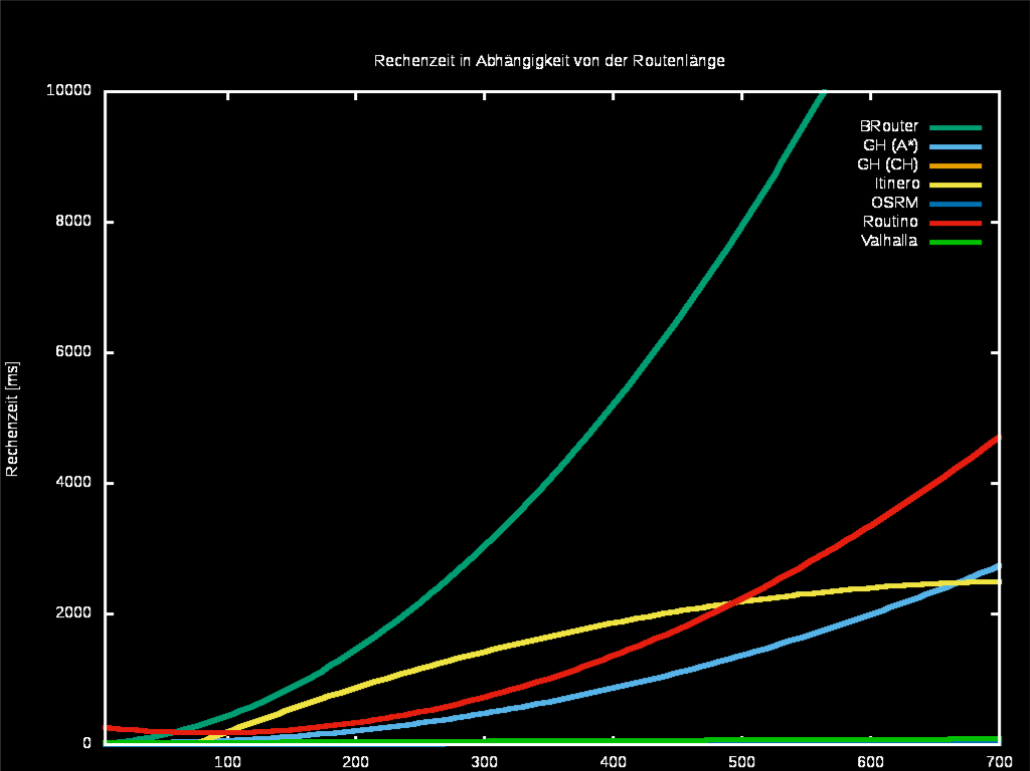
\includegraphics[width=1.0\textwidth]{img/routing_comparison_01}
\captionof{figure}{Comparison of all open source Routing Engines}\label{fig:routing_comparison_01}
\end{figure}
\begin{figure}[H]
\centering
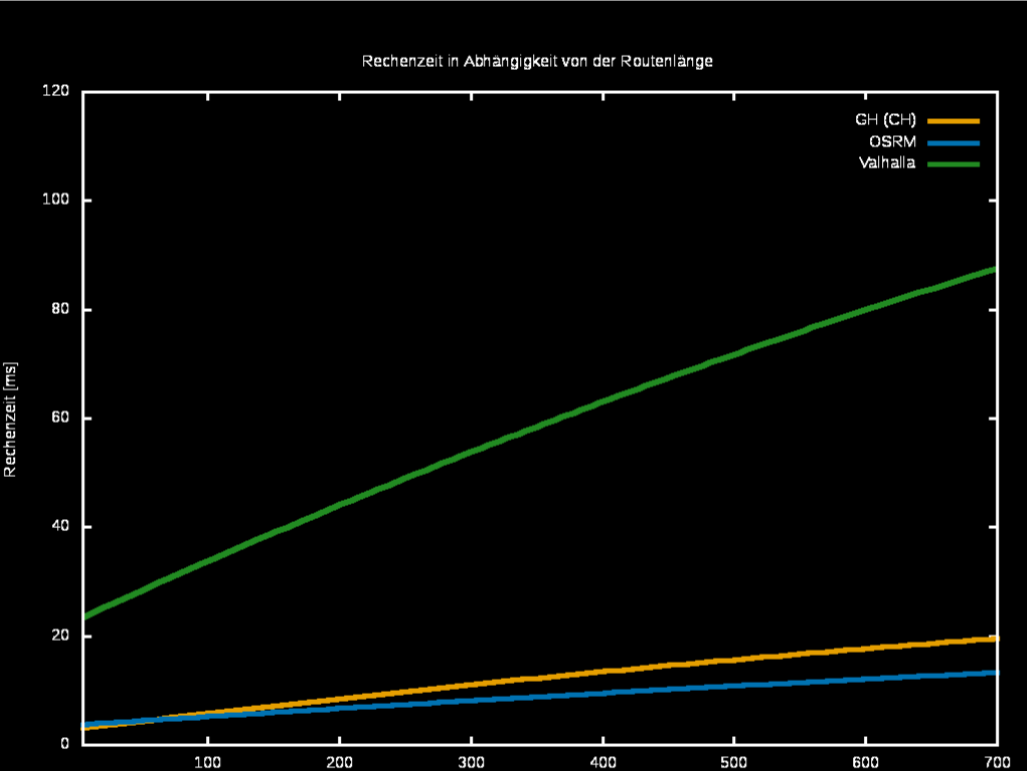
\includegraphics[width=1.0\textwidth]{img/routing_comparison_02}
\captionof{figure}{Comparison of fastest open source Routing Engines}\label{fig:routing_comparison_02}
\end{figure}
As can be seen, Graphopper (GH), Open Source Routing Machine (OSRM) and Valhalla are the best-performing open source routing engines. Therefore, a closer look shall be taken at these three:


TODO Tabelle einfügen (LIZENZ, OS, ALGORITHMS, ETC)






Unfortunately OSRM has very high hardware requirements\citep{J.2017}. Preprocessing the car profile requires at least 175 GB of RAM and 280 GB of disk space. Additionally, 35 GB are needed for the planet osm.pbf (Openstreetmaps) and 40 to 50 GB for the generated data files. For the foot profile 248 GB of RAM are needed. During runtime the car profile requires around 64 GB of RAM, the foot profile even more. Basically OSRM loads the preprocessed files completely into RAM\citep{J.2017}. The project team's VM had only 64 GB of RAM and half of it was already used for Pelias and Elasticsearch. Hence, it was not possible to install OSRM and evaluate it completely.

\subsection{Graphopper vs Valhalla}
We performed an in-depth comparison of the time it takes for routing from one point to another with Graphhopper and Valhalla. The results of these test series can be seen in the table \ref{GHvsVH}.
%
\begin{table}
\centering
\begin{tabular}[H]{@{}p{0.5cm}|p{1.5cm}|p{2.3cm}|p{2.3cm}|p{2.3cm}|p{2.3cm}|p{2.3cm}|p{2.3cm}}
                                       &                           & \textbf{Route 1} & \textbf{Route 2} & \textbf{Route 3} & \textbf{Route 4} & \textbf{Route 5} & \textbf{Route 6}  \\ \hline
                                       & \textbf{Route from}       & Catania, Italy Latitude: 37.502236 Longitude: 15.08738 & 1100-148 Lisbon, Portugal Latitude: 38.707751 Longitude: -9.136592 & Ulm, Baden-Württemberg, Germany Latitude: 48.3974 Longitude: 9.993434 & Paris, France Latitude: 48.856697 Longitude: 2.351462 & 37011 Bardolino VR, Italy Latitude: 45.553553 Longitude: 10.637519 & North Cape, E 69, Norway Latitude: 71.169951 Longitude: 25.785889 \\ \hline
                                       & \textbf{Route to}         &  1357 Copenhagen, Denmark Latitude: 55.686724 Longitude: 12.570072 & Warsaw, Warszawa, Poland Latitude: 52.231924 Longitude: 21.006727 & Munich, Bavaria, Germany Latitude: 48.137108 Longitude: 11.575382 & Venice, Venezia, Italy Latitude: 45.437191 Longitude: 12.33459 & Gunterstraße 8, 70191 Stuttgart, Germany Latitude: 48.806576 Longitude: 9.178105 & 89032 Bianco RC, Italy Latitude: 38.087176 Longitude: 16.148511 \\ \hline
\multirow{3}{*}{\textbf{GH}} & \textbf{first try}        & real 0m0.735s user 0m0.013s sys 0m0.006s & real 0m0.300s user 0m0.016s sys 0m0.006s & real 0m0.031s user 0m0.004s sys 0m0.011s & real 0m0.083s user 0m0.016s sys 0m0.000s & - & real 0m0.261s user 0m0.013s sys 0m0.011s \\ \hline
                                       & \textbf{second try}       & real 0m0.188s user 0m0.019s sys 0m0.000s & real 0m0.407s user 0m0.014s sys 0m0.005s & real 0m0.022s user 0m0.014s sys 0m0.000s & real 0m0.042s user 0m0.014s sys 0m0.004s & - & real 0m0.216s user 0m0.024s sys 0m0.004s \\ \hline
                                       & \textbf{distance (in km)} & 2753 & 3318 & 139 & 1113 & - & 5112 \\ \hline
\multirow{3}{*}{\textbf{VH}}    & \textbf{first try}        & real 0m2.098s user 0m0.014s sys 0m0.013s & real 0m4.805s user 0m0.013s sys 0m0.021s & real 0m0.668s user 0m0.012s sys 0m0.006s & real 0m3.121s user 0m0.020s sys 0m0.003s & real 0m1.037s user 0m0.012s sys 0m0.009s & real 0m1.784s user 0m0.030s sys 0m0.003s \\ \hline
                                       & \textbf{second try}       & real 0m0.279s user 0m0.018s sys 0m0.008s & real 0m0.498s user 0m0.030s sys 0m0.003s & real 0m0.083s user 0m0.014s sys 0m0.004s & real 0m0.571s user 0m0.014s sys 0m0.008s & real 0m0.086s user 0m0.017s sys 0m0.005s & real 0m0.607s user 0m0.026s sys 0m0.008s \\ \hline
                                       & \textbf{distance (in km)} & 2682 & 3408 & 141 & 1116 & 579 & 4996 %\\ \hline
%                                       & \textbf{remark}           &  &  &  &  & Coordinates of the starting point in the middle of lake garda. Graphhopper couldn’t calculate a route & 
\end{tabular}
\caption{Graphhopper vs. Valhalla test row \label{GHvsVH}}
\end{table}

The API requests were executed directly on the Graphhopper and Valhalla host machines using the command line programs time and curl.
We can see, that Graphhopper compared to Valhalla does a significantly better job when calculating a new route for the very first time. The execution time in Valhalla varies from the first calculation to the second calculation by up to the factor of ten. This means calculating a route or part of it, which has already been calculated before, the execution time is almost ten times faster compared to the first calculation. Valhalla achieves this with caching routes in RAM. Graphhopper however has a problem, if there is no road or street to be routed from or to for a given start- or end-point. Valhalla in this case just takes the closest routable point instead.  Choosing one routing engine over the other depends on the goal which should be achieved. For fastest execution time (not regarding first or second execution) Graphhopper fits best. If you want to make sure, that you receive a route whichever point you calculate from or to, then it is recommended to use Valhalla.

\subsection{Conclusion}
OSRM is the fastest routing engine on the open-source market. But because of the very high memory requirements of OSRM it is not suitable for the use-case of our project and the cost/benefit-factor is too low. Valhalla would be a good alternative to Graphhopper, because it is compared to other routing engines nearly as fast as Graphhopper and is designed to work with Openstreetmaps-data and also recommended by the Pelias developers to be used in connection with Pelias as a geocoder. Also Valhalla is capable of routing from or to points, which do not have a road or street directly nearby. A very valuable feature especially for two-digit postcode centroids, which Graphhopper does not have. However, in this early state of the project Graphhopper totally fits all the needs and therefore there is no need in replacing Graphhopper with Valhalla.


% vim:ft=tex

\section{Valhalla}
Valhalla was installed and configured according to the official documentation on Github \cite{Knisely2019}.
Tiles and polylines were calculated using the same openstreetmaps pbf file (Europe) which was already used for Pelias. Routing can be achieved by querying Valhalla’s api:

\begin{lstlisting}[language=bash,breaklines=true]
curl http://141.59.29.110:8002/route --data '{"locations":[{"lat":48.1331,"lon":11.6046,"type":"break"},{"lat":47.9419,"lon":11.2759,"type":"break"}],"costing":"auto","directions_options":{"units":"km"}}' | jq '.'
\end{lstlisting}

Result:

\begin{lstlisting}[language=json,breaklines=true]
    "summary": {
      "max_lon": 11.605507,
      "max_lat": 48.133167,
      "time": 2397,
      "length": 38.536,
      "min_lat": 47.943157,
      "min_lon": 11.260186
    },
    "locations": [
      {
        "original_index": 0,
        "type": "break",
        "lon": 11.6046,
        "lat": 48.133099,
        "side_of_street": "right"
      },
      {
        "original_index": 1,
        "type": "break",
        "lon": 11.2759,
        "lat": 47.941898,
        "side_of_street": "right"
      }
    ]
\end{lstlisting}

The complete output and routing instructions are in the appendix page \pageref{VRO}.

\newpage
\bibliographystyle{plain}
\bibliography{./bibtex/junior_report}
\renewcommand{\listfigurename}{B Illustration Directory}
\listoffigures

\begin{appendices}
  \chapter{Valhalla Routing}
  % \section{Valhalla Routing Output} \label{VRO}
\begin{lstlisting}[language=json,breaklines=true]
{
  "trip": {
    "language": "en-US",
    "status": 0,
    "units": "kilometers",
    "status_message": "Found route between points",
    "legs": [
      {
        "summary": {
          "max_lon": 11.605507,
          "max_lat": 48.133167,
          "time": 2397,
          "length": 38.536,
          "min_lat": 47.943157,
          "min_lon": 11.260186
        },
        "maneuvers": [
          {
            "travel_type": "car",
            "street_names": [
              "Kirchenstrasse"
            ],
            "verbal_pre_transition_instruction": "Drive east on Kirchenstrasse for 30 meters. Then Turn right onto Elsaesser Strasse.",
            "instruction": "Drive east on Kirchenstrasse.",
            "end_shape_index": 2,
            "type": 2,
            "time": 15,
            "verbal_multi_cue": true,
            "length": 0.033,
            "begin_shape_index": 0,
            "travel_mode": "drive"
          },
          {
            "travel_type": "car",
            "travel_mode": "drive",
            "verbal_pre_transition_instruction": "Turn right onto Elsaesser Strasse.",
            "verbal_transition_alert_instruction": "Turn right onto Elsaesser Strasse.",
            "length": 0.424,
            "instruction": "Turn right onto Elsaesser Strasse.",
            "end_shape_index": 21,
            "type": 10,
            "time": 107,
            "verbal_post_transition_instruction": "Continue for 400 meters.",
            "street_names": [
              "Elsaesser Strasse"
            ],
            "begin_shape_index": 2
          },
          {
            "travel_type": "car",
            "travel_mode": "drive",
            "verbal_pre_transition_instruction": "Turn right onto Orleansstrasse.",
            "verbal_transition_alert_instruction": "Turn right onto Orleansstrasse.",
            "length": 0.887,
            "instruction": "Turn right onto Orleansstrasse.",
            "end_shape_index": 57,
            "type": 10,
            "time": 149,
            "verbal_post_transition_instruction": "Continue for 900 meters.",
            "street_names": [
              "Orleansstrasse"
            ],
            "begin_shape_index": 21
          },
          {
            "travel_type": "car",
            "verbal_pre_transition_instruction": "Continue on Auerfeldstrasse for 200 meters.",
            "verbal_transition_alert_instruction": "Continue on Auerfeldstrasse.",
            "length": 0.161,
            "instruction": "Continue on Auerfeldstrasse.",
            "end_shape_index": 68,
            "type": 8,
            "time": 42,
            "street_names": [
              "Auerfeldstrasse"
            ],
            "begin_shape_index": 57,
            "travel_mode": "drive"
          },
          {
            "travel_type": "car",
            "verbal_pre_transition_instruction": "Continue on Welfenstrasse for 700 meters.",
            "verbal_transition_alert_instruction": "Continue on Welfenstrasse.",
            "length": 0.708,
            "instruction": "Continue on Welfenstrasse.",
            "end_shape_index": 100,
            "type": 8,
            "time": 105,
            "street_names": [
              "Welfenstrasse"
            ],
            "begin_shape_index": 68,
            "travel_mode": "drive"
          },
          {
            "travel_type": "car",
            "travel_mode": "drive",
            "verbal_pre_transition_instruction": "Turn left onto Regerstrasse.",
            "verbal_transition_alert_instruction": "Turn left onto Regerstrasse.",
            "length": 0.155,
            "instruction": "Turn left onto Regerstrasse.",
            "end_shape_index": 113,
            "type": 15,
            "time": 18,
            "verbal_post_transition_instruction": "Continue for 200 meters.",
            "street_names": [
              "Regerstrasse"
            ],
            "begin_shape_index": 100
          },
          {
            "travel_type": "car",
            "verbal_pre_transition_instruction": "Continue on Tegernseer Landstrasse for 600 meters.",
            "verbal_transition_alert_instruction": "Continue on Tegernseer Landstrasse.",
            "length": 0.631,
            "instruction": "Continue on Tegernseer Landstrasse.",
            "end_shape_index": 167,
            "type": 8,
            "time": 77,
            "street_names": [
              "Tegernseer Landstrasse"
            ],
            "begin_shape_index": 113,
            "travel_mode": "drive"
          },
          {
            "travel_type": "car",
            "travel_mode": "drive",
            "verbal_pre_transition_instruction": "Turn right onto Ichostrasse.",
            "verbal_transition_alert_instruction": "Turn right onto Ichostrasse.",
            "length": 0.183,
            "instruction": "Turn right onto Ichostrasse.",
            "end_shape_index": 179,
            "type": 10,
            "time": 27,
            "verbal_post_transition_instruction": "Continue for 200 meters.",
            "street_names": [
              "Ichostrasse"
            ],
            "begin_shape_index": 167
          },
          {
            "travel_type": "car",
            "travel_mode": "drive",
            "verbal_multi_cue": true,
            "verbal_pre_transition_instruction": "Bear left to stay on Ichostrasse. Then Bear left onto Martin-Luther-Strasse.",
            "verbal_transition_alert_instruction": "Bear left to stay on Ichostrasse.",
            "length": 0.045,
            "instruction": "Bear left to stay on Ichostrasse.",
            "end_shape_index": 186,
            "type": 16,
            "time": 6,
            "verbal_post_transition_instruction": "Continue for 50 meters.",
            "street_names": [
              "Ichostrasse"
            ],
            "begin_shape_index": 179
          },
          {
            "travel_type": "car",
            "travel_mode": "drive",
            "verbal_pre_transition_instruction": "Bear left onto Martin-Luther-Strasse.",
            "verbal_transition_alert_instruction": "Bear left onto Martin-Luther-Strasse.",
            "length": 0.347,
            "instruction": "Bear left onto Martin-Luther-Strasse.",
            "end_shape_index": 211,
            "type": 16,
            "time": 46,
            "verbal_post_transition_instruction": "Continue for 300 meters.",
            "street_names": [
              "Martin-Luther-Strasse"
            ],
            "begin_shape_index": 186
          },
          {
            "travel_type": "car",
            "travel_mode": "drive",
            "verbal_pre_transition_instruction": "Continue on Tegernseer Landstrasse for 100 meters. Then Turn right onto Candidstrasse.",
            "verbal_transition_alert_instruction": "Continue on Tegernseer Landstrasse.",
            "length": 0.121,
            "instruction": "Continue on Tegernseer Landstrasse.",
            "end_shape_index": 219,
            "type": 8,
            "time": 13,
            "verbal_multi_cue": true,
            "street_names": [
              "Tegernseer Landstrasse"
            ],
            "begin_shape_index": 211
          },
          {
            "travel_type": "car",
            "travel_mode": "drive",
            "verbal_pre_transition_instruction": "Turn right onto Candidstrasse.",
            "verbal_transition_alert_instruction": "Turn right onto Candidstrasse.",
            "length": 0.933,
            "instruction": "Turn right onto Candidstrasse.",
            "end_shape_index": 289,
            "type": 10,
            "time": 97,
            "verbal_post_transition_instruction": "Continue for 900 meters.",
            "street_names": [
              "Candidstrasse"
            ],
            "begin_shape_index": 219
          },
          {
            "travel_type": "car",
            "travel_mode": "drive",
            "verbal_pre_transition_instruction": "Take the B 2R ramp on the left.",
            "verbal_transition_alert_instruction": "Take the B 2R ramp on the left.",
            "instruction": "Take the B 2R ramp on the left.",
            "end_shape_index": 297,
            "type": 19,
            "time": 9,
            "street_names": [
              "Candidstrasse"
            ],
            "begin_shape_index": 289,
            "length": 0.124,
            "sign": {
              "exit_branch_elements": [
                {
                  "text": "B 2R"
                }
              ]
            }
          },
          {
            "travel_type": "car",
            "travel_mode": "drive",
            "verbal_pre_transition_instruction": "Merge onto B 2R.",
            "begin_street_names": [
              "B 2R",
              "Candidstrasse"
            ],
            "verbal_post_transition_instruction": "Continue for 3 kilometers.",
            "instruction": "Merge onto B 2R.",
            "end_shape_index": 354,
            "type": 25,
            "time": 182,
            "street_names": [
              "B 2R"
            ],
            "length": 3.038,
            "begin_shape_index": 297
          },
          {
            "travel_type": "car",
            "travel_mode": "drive",
            "verbal_pre_transition_instruction": "Take the A 95 ramp on the right toward Garmisch-Partenkirchen, Forstenried.",
            "verbal_transition_alert_instruction": "Take the A 95 ramp on the right.",
            "instruction": "Take the A 95 ramp on the right toward Garmisch-Partenkirchen/Forstenried/Fuerstenried/Grosshadern.",
            "end_shape_index": 360,
            "type": 18,
            "time": 14,
            "street_names": [
              "Heckenstallertunnel"
            ],
            "begin_shape_index": 354,
            "length": 0.305,
            "sign": {
              "exit_toward_elements": [
                {
                  "text": "Garmisch-Partenkirchen"
                },
                {
                  "text": "Forstenried"
                },
                {
                  "text": "Fuerstenried"
                },
                {
                  "text": "Grosshadern"
                }
              ],
              "exit_branch_elements": [
                {
                  "text": "A 95"
                }
              ]
            }
          },
          {
            "travel_type": "car",
            "verbal_pre_transition_instruction": "Keep right at the fork. Then Bear right onto Luise-Kiesselbach-Platz.",
            "verbal_transition_alert_instruction": "Keep right at the fork.",
            "length": 0.025,
            "instruction": "Keep right at the fork.",
            "end_shape_index": 363,
            "type": 23,
            "time": 6,
            "verbal_multi_cue": true,
            "begin_shape_index": 360,
            "travel_mode": "drive"
          },
          {
            "travel_type": "car",
            "travel_mode": "drive",
            "verbal_multi_cue": true,
            "verbal_pre_transition_instruction": "Bear right onto Luise-Kiesselbach-Platz. Then Take the ramp on the left toward A 95.",
            "verbal_transition_alert_instruction": "Bear right onto Luise-Kiesselbach-Platz.",
            "length": 0.079,
            "instruction": "Bear right onto Luise-Kiesselbach-Platz.",
            "end_shape_index": 367,
            "type": 9,
            "time": 13,
            "verbal_post_transition_instruction": "Continue for 80 meters.",
            "street_names": [
              "Luise-Kiesselbach-Platz"
            ],
            "begin_shape_index": 363
          },
          {
            "travel_type": "car",
            "travel_mode": "drive",
            "verbal_pre_transition_instruction": "Take the ramp on the left toward A 95. Then Keep left at the fork.",
            "verbal_transition_alert_instruction": "Take the ramp on the left toward A 95.",
            "instruction": "Take the ramp on the left toward A 95.",
            "end_shape_index": 369,
            "type": 19,
            "time": 5,
            "verbal_multi_cue": true,
            "begin_shape_index": 367,
            "length": 0.037,
            "sign": {
              "exit_toward_elements": [
                {
                  "text": "A 95"
                }
              ]
            }
          },
          {
            "travel_type": "car",
            "verbal_pre_transition_instruction": "Keep left at the fork. Then Take the B 2 ramp on the left.",
            "verbal_transition_alert_instruction": "Keep left at the fork.",
            "length": 0.087,
            "instruction": "Keep left at the fork.",
            "end_shape_index": 374,
            "type": 24,
            "time": 34,
            "verbal_multi_cue": true,
            "begin_shape_index": 369,
            "travel_mode": "drive"
          },
          {
            "travel_type": "car",
            "verbal_pre_transition_instruction": "Take the B 2 ramp on the left.",
            "verbal_transition_alert_instruction": "Take the B 2 ramp on the left.",
            "instruction": "Take the B 2 ramp on the left.",
            "end_shape_index": 381,
            "type": 19,
            "time": 25,
            "begin_shape_index": 374,
            "length": 0.264,
            "sign": {
              "exit_branch_elements": [
                {
                  "text": "B 2"
                }
              ]
            },
            "travel_mode": "drive"
          },
          {
            "travel_type": "car",
            "verbal_pre_transition_instruction": "Merge onto A 95.",
            "verbal_post_transition_instruction": "Continue for 1.2 kilometers.",
            "instruction": "Merge onto A 95.",
            "end_shape_index": 387,
            "type": 25,
            "time": 81,
            "street_names": [
              "A 95"
            ],
            "length": 1.159,
            "begin_shape_index": 381,
            "travel_mode": "drive"
          },
          {
            "travel_type": "car",
            "travel_mode": "drive",
            "verbal_pre_transition_instruction": "Continue on B 2 for 80 meters. Then Continue on A 95.",
            "verbal_transition_alert_instruction": "Continue on B 2.",
            "length": 0.078,
            "instruction": "Continue on B 2.",
            "end_shape_index": 388,
            "type": 8,
            "time": 3,
            "verbal_multi_cue": true,
            "street_names": [
              "B 2"
            ],
            "begin_shape_index": 387
          },
          {
            "travel_type": "car",
            "verbal_pre_transition_instruction": "Continue on A 95 for 11.5 kilometers.",
            "verbal_transition_alert_instruction": "Continue on A 95.",
            "length": 11.482,
            "instruction": "Continue on A 95.",
            "end_shape_index": 486,
            "type": 8,
            "time": 461,
            "street_names": [
              "A 95"
            ],
            "begin_shape_index": 388,
            "travel_mode": "drive"
          },
          {
            "travel_type": "car",
            "verbal_pre_transition_instruction": "Take exit 4 on the right onto A 9 52 toward Starnberg.",
            "verbal_transition_alert_instruction": "Take exit 4 on the right.",
            "instruction": "Take exit 4 on the right onto A 952 toward Starnberg.",
            "end_shape_index": 510,
            "type": 20,
            "time": 51,
            "begin_shape_index": 486,
            "length": 1.172,
            "sign": {
              "exit_name_elements": [
                {
                  "text": "Dreieck Starnberg"
                }
              ],
              "exit_toward_elements": [
                {
                  "text": "Starnberg"
                }
              ],
              "exit_branch_elements": [
                {
                  "consecutive_count": 1,
                  "text": "A 952"
                }
              ],
              "exit_number_elements": [
                {
                  "text": "4"
                }
              ]
            },
            "travel_mode": "drive"
          },
          {
            "travel_type": "car",
            "verbal_pre_transition_instruction": "Merge onto A 9 52.",
            "verbal_post_transition_instruction": "Continue for 4 kilometers.",
            "instruction": "Merge onto A 952.",
            "end_shape_index": 556,
            "type": 25,
            "time": 150,
            "street_names": [
              "A 952"
            ],
            "length": 3.984,
            "begin_shape_index": 510,
            "travel_mode": "drive"
          },
          {
            "travel_type": "car",
            "verbal_pre_transition_instruction": "Continue on B 2 for a half kilometer.",
            "verbal_transition_alert_instruction": "Continue on B 2.",
            "length": 0.458,
            "instruction": "Continue on B 2.",
            "end_shape_index": 563,
            "type": 8,
            "time": 28,
            "street_names": [
              "B 2"
            ],
            "begin_shape_index": 556,
            "travel_mode": "drive"
          },
          {
            "travel_type": "car",
            "travel_mode": "drive",
            "verbal_pre_transition_instruction": "Continue on Muenchner Strasse for 1.1 kilometers.",
            "begin_street_names": [
              "B 2",
              "Muenchner Strasse"
            ],
            "verbal_transition_alert_instruction": "Continue on Muenchner Strasse.",
            "length": 1.14,
            "instruction": "Continue on Muenchner Strasse.",
            "end_shape_index": 603,
            "type": 8,
            "time": 91,
            "street_names": [
              "Muenchner Strasse"
            ],
            "begin_shape_index": 563
          },
          {
            "travel_type": "car",
            "travel_mode": "drive",
            "verbal_pre_transition_instruction": "Continue on B 2 for 3.1 kilometers.",
            "begin_street_names": [
              "Hauptstrasse",
              "B 2"
            ],
            "verbal_transition_alert_instruction": "Continue on B 2.",
            "length": 3.086,
            "instruction": "Continue on B 2.",
            "end_shape_index": 679,
            "type": 8,
            "time": 189,
            "street_names": [
              "B 2"
            ],
            "begin_shape_index": 603
          },
          {
            "travel_type": "car",
            "verbal_pre_transition_instruction": "Enter the roundabout and take the 2nd exit.",
            "verbal_transition_alert_instruction": "Enter the roundabout and take the 2nd exit.",
            "length": 0.083,
            "instruction": "Enter the roundabout and take the 2nd exit.",
            "end_shape_index": 689,
            "type": 26,
            "time": 4,
            "begin_shape_index": 679,
            "roundabout_exit_count": 2,
            "travel_mode": "drive"
          },
          {
            "travel_type": "car",
            "travel_mode": "drive",
            "verbal_pre_transition_instruction": "Exit the roundabout onto Weilheimer Strasse, B 2.",
            "begin_street_names": [
              "Weilheimer Strasse",
              "B 2"
            ],
            "verbal_post_transition_instruction": "Continue on B 2 for 5.8 kilometers.",
            "instruction": "Exit the roundabout onto Weilheimer Strasse/B 2. Continue on B 2.",
            "end_shape_index": 800,
            "type": 27,
            "time": 242,
            "street_names": [
              "B 2"
            ],
            "length": 5.768,
            "begin_shape_index": 689
          },
          {
            "travel_type": "car",
            "travel_mode": "drive",
            "verbal_pre_transition_instruction": "Bear right onto Starnberger Strasse.",
            "verbal_transition_alert_instruction": "Bear right onto Starnberger Strasse.",
            "length": 0.237,
            "instruction": "Bear right onto Starnberger Strasse.",
            "end_shape_index": 808,
            "type": 9,
            "time": 17,
            "verbal_post_transition_instruction": "Continue for 200 meters.",
            "street_names": [
              "Starnberger Strasse"
            ],
            "begin_shape_index": 800
          },
          {
            "travel_type": "car",
            "travel_mode": "drive",
            "verbal_multi_cue": true,
            "verbal_pre_transition_instruction": "Bear left onto Feldafinger Strasse. Then Bear left to stay on Feldafinger Strasse.",
            "verbal_transition_alert_instruction": "Bear left onto Feldafinger Strasse.",
            "length": 0.108,
            "instruction": "Bear left onto Feldafinger Strasse.",
            "end_shape_index": 816,
            "type": 16,
            "time": 9,
            "verbal_post_transition_instruction": "Continue for 100 meters.",
            "street_names": [
              "Feldafinger Strasse"
            ],
            "begin_shape_index": 808
          },
          {
            "travel_type": "car",
            "travel_mode": "drive",
            "verbal_multi_cue": true,
            "verbal_pre_transition_instruction": "Bear left to stay on Feldafinger Strasse. Then Bear right to stay on Feldafinger Strasse.",
            "verbal_transition_alert_instruction": "Bear left to stay on Feldafinger Strasse.",
            "length": 0.101,
            "instruction": "Bear left to stay on Feldafinger Strasse.",
            "end_shape_index": 820,
            "type": 16,
            "time": 9,
            "verbal_post_transition_instruction": "Continue for 100 meters.",
            "street_names": [
              "Feldafinger Strasse"
            ],
            "begin_shape_index": 816
          },
          {
            "travel_type": "car",
            "travel_mode": "drive",
            "verbal_pre_transition_instruction": "Bear right to stay on Feldafinger Strasse.",
            "verbal_transition_alert_instruction": "Bear right to stay on Feldafinger Strasse.",
            "length": 0.313,
            "instruction": "Bear right to stay on Feldafinger Strasse.",
            "end_shape_index": 830,
            "type": 9,
            "time": 21,
            "verbal_post_transition_instruction": "Continue for 300 meters.",
            "street_names": [
              "Feldafinger Strasse"
            ],
            "begin_shape_index": 820
          },
          {
            "travel_type": "car",
            "travel_mode": "drive",
            "begin_shape_index": 830,
            "time": 51,
            "type": 8,
            "end_shape_index": 852,
            "instruction": "Continue.",
            "length": 0.78,
            "verbal_transition_alert_instruction": "Continue.",
            "time": 51,
            "type": 8,
            "end_shape_index": 852,
            "instruction": "Continue.",
            "length": 0.78,
            "verbal_transition_alert_instruction": "Continue.",
            "verbal_pre_transition_instruction": "Continue for 800 meters."
          },
          {
            "travel_type": "car",
            "travel_mode": "drive",
            "begin_shape_index": 852,
            "time": 0,
            "type": 5,
            "end_shape_index": 852,
            "instruction": "Your destination is on the right.",
            "length": 0,
            "verbal_transition_alert_instruction": "Your destination will be on the right.",
            "verbal_pre_transition_instruction": "Your destination is on the right."
          }
        ]
      }
    ],
    "summary": {
      "max_lon": 11.605507,
      "max_lat": 48.133167,
      "time": 2397,
      "length": 38.536,
      "min_lat": 47.943157,
      "min_lon": 11.260186
    },
    "locations": [
      {
        "original_index": 0,
        "type": "break",
        "lon": 11.6046,
        "lat": 48.133099,
        "side_of_street": "right"
      },
      {
        "original_index": 1,
        "type": "break",
        "lon": 11.2759,
        "lat": 47.941898,
        "side_of_street": "right"
      }
    ]
  }
}
\end{lstlisting}
  \chapter{bliblablubb}
\end{appendices}

\end{document}
